\documentclass[12pt]{article}
\usepackage[cm]{fullpage}
\usepackage{listings}
\usepackage{color}
\usepackage{xcolor}
\usepackage{textpos}
\usepackage{amssymb,latexsym}
\usepackage{amsmath}
\usepackage{xltxtra,xunicode,xgreek}
\usepackage[colorlinks=true, linkcolor = blue, citecolor=blue]{hyperref}
\usepackage[ddmmyyyy]{datetime}
\usepackage{float}
\usepackage{textcomp}
\usepackage{url} 
\usepackage{turnstile}
\usepackage{xcolor,colortbl}


\definecolor{gray}{gray}{0.89}
\definecolor{ablack}{HTML}{25383C}
\setmainfont[Mapping=tex-text]{CMU Concrete}
\setmonofont{Courier New}
\newcommand{\tab}{\hspace*{2em}}
\newcommand{\rom}[1]{\uppercase\expandafter{\romannumeral #1\relax}}
\setlength{\parindent}{0pt}

\newcommand{\Llama}{\textit{Llama }}

\usepackage{caption}
\DeclareCaptionFont{white}{\color{white}}
\DeclareCaptionFormat{listing}{\colorbox{gray}{\parbox{\textwidth}{#1#2#3}}}
\captionsetup[lstlisting]{format=listing,labelfont=white,textfont=white}
%\renewcommand\listingscaption{Κώδικας}
\renewcommand{\arraystretch}{1.5}


\begin{document}
\begin{titlepage}
\begin{center}


\includegraphics[scale=0.3]{pyrforos.jpg}\\
ΕΘΝΙΚΟ ΜΕΤΣΟΒΙΟ ΠΟΛΥΤΕΧΝΕΙΟ \\
ΣΧΟΛΗ ΗΛΕΚΤΡΟΛΟΓΩΝ ΜΗΧΑΝΙΚΩΝ KΑΙ ΜΗΧΑΝΙΚΩΝ ΥΠΟΛΟΓΙΣΤΩΝ \\ 
\vspace{0.5em}

\medskip 

\def\doubleline{

    \vspace{0.1em}
    \line(1,0){530}\

    \vspace{-1.5em}
    \line(1,0){530}

}
\doubleline
\vspace{1.3em}

{\large \textbf{Μεταγλωτιστές}\\
 \medskip
8ο εξάμηνο, Ακαδημαϊκή περίοδος 2012 \\ \bigskip \medskip}

\vspace{1.5em}
{\LARGE \textbf{Υλοποίηση της γλώσσας \Llama\\}}
\vspace{1cm}
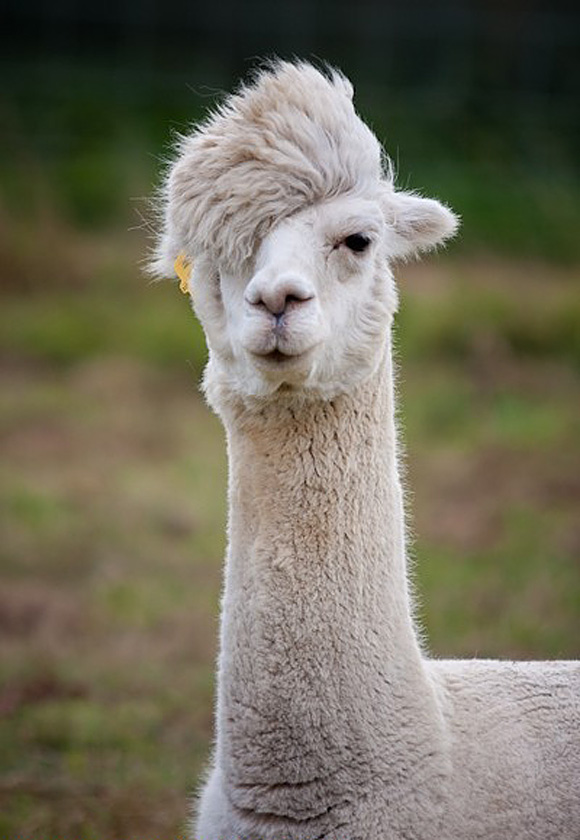
\includegraphics[scale=0.4]{llama.jpg}\\
\vfill
\begin{tabular}{l l}
Kωνσταντίνος Αθανασίου & 03108132\\
Νίκος Γιανναράκης & 03108054 \\
Ζωή Παρασκευοπούλου & 03108152 \\
\end{tabular}\\
\bigskip
\today
\end{center}
\end{titlepage}
\tableofcontents

\pagebreak

\section{Εισαγωγή}
H \Llama είναι μια γλώσσα η οποία συνδυάζει στοιχεία συναρτησιακού και προστακτικού προγραμματισμού και συντακτικά μοιάζει αρκετά με τη γλώσσα Caml. Η εργασία έχει υλοποιηθεί στη γλώσσα OCaml. Αναλυτικά οι προδιαγραφές τις γλώσσας βρίσκονται \href{http://courses.softlab.ntua.gr/compilers/2012a/llama2012.pdf}{εδώ}
\section{Υλοποίση}
Στην ενότητα αυτή θα παρουσιάσουμε συνοπτικά κάποια βασικά στοιχεία της υλοποίησης.
\subsection{Συντακτικός και Γραμματικός Αναλυτής}
Για τον συντακτικό αναλυτή χρησιμοποιήθηκε το εργαλείο \href{http://courses.softlab.ntua.gr/compilers/2012a/ocamlyacc-tutorial.pdf}{Ocamllex} και για τον γραμματικό     αναλυτή το εργαλείο \href{http://courses.softlab.ntua.gr/compilers/2012a/ocamlyacc-tutorial.pdf}{Ocamlyacc}.
\subsection{Σημασιολογική Ανάλυση}
Ο σημασιολογικός αναλυτής της \Llama αποτελείται κυρίως από την εξαγωγή τύπων καθώς και από τον έλεγχο κάποιων επιπλέον περιορισμών.
\subsubsection{Εξαγωγή Τύπων}
Η εξαγωγή τύπων βασίζεται στην παραγωγή περιορισμών, υπό τη μορφή εξισώσεων τύπων, κατά τη διάσχιση του ast, κάθε άγωστος τύπος αναπαριστάται από μια μοναδική μεταβλητή τύπου. Στο τέλος της διάσχισης καλείται η συνάρτηση unify η οποία λύνει τους περιορισμούς αναθέτει σε κάθε μεταβλητή τύπου έναν γνωστό τύπο. Σε περίπτωση όπου οι περιορισμοί δεν είναι επιλύσιμοι επιστρέφεται μήνυμα λάθους το οποίο επισημαίνει του δύο τύπους που δεν μπορούν να ενοποιηθούν.


Στην γλώσσα Llama οι τελεστές σύγκρισης υποστηρίζονται μόνο για τους τύπους int, float και char. Προκειμένου να ελέγξουμε στατικά αυτόν τον περιορισμό δημιουργούμε έναν καινούριο τύπο ord που αναπαριστά τους τύπους που υποστηρίζουν τελεστές διάταξης. Έτσι προκύπτει ο παρακάτω κανόνας τυποποίησης:

$$\frac{\Gamma  \vdash e_1 : ord \;\;\;\; \Gamma  \vdash e_2 : ord  }{\Gamma  \vdash e_1 \diamond e_2 : bool,\diamond \in \lbrace <,>, \leq, \geq\rbrace}$$


Μετά την δημιουργία των αντιστοίχων constraints η συνάρτηση unify συσσωρεύει τούς τύπους που προκύπτει από τους περιορισμούς ότι πρέπει να υποστηρίζουν διάταξη και αφού λύσει όλους τους περιορισμούς και εφαρμόσει όλες τις αντικαταστάσεις που προκύπτουν για τις μεταβλητές τύπων, ελέγχει αν οι συσσωρευμένοι τύποι είναι από τους 3 τύπους που υποστηρίζουν διάταξη, διαφορετικά γυρνάει μήνυμα λάθους. Με ανάλογο τρόπο ελέγχεται ότι ο τύπος επιστροφής των συναρτήσεων δεν είναι τύπος συνάρτησης κάτι που απαγορεύεται στη \Llama. 

%% TODO TODO TODΟ elegxos sunarthshs pou elegxei ta ord ston compiler einai lathos

\subsubsection{Έλεγχος επιπλέον περιορισμών}





\subsection{Πίνακες}
\subsection{Συναρτησεις Υψηλής Τάξης}
\subsection{Τύποι Οριζόμενοι από τον Προγραμματιστή}
\subsubsection{Αναπαράσταση}
\subsubsection{Υλοποίηση Δομικής Ισότητας}
\subsection{Control Flow Graph}
Για την υλοποίηση του γράφου ροής ελέγχου αρχικά χωρίσαμε της τετράδες του ενδιάμεσου κώδικα σε Blocks έτσι ώστε να υπάρχουν άλματα μόνο ως προς την πρώτη εντολή κάθε Block και οι εντολές άλματος
(γενικότερα οι εντολές αλλαγής ροής του προγράμματος) να βρίσκονται μόνο στο τέλος κάποιου Block. Σε κάθε Block πέρα από τις αριθμημένες τετράδες που το αποτελούν, μέσω ενός record αποθηκεύουμε και επιπλέον πληροφορίες που διευκολύνουν την ανάλυση του προγράμματος σε αυτή τη μορφή, όπως για παράδειγμα το αν ορίζεται κάποια συνάρτηση μέσα σε αυτό το Block ή σε ποια συνάρτηση ανήκουν οι τετράδες του κάθε Block και αν κάποιο Block περιλαμβάνει το τέλος μίας συνάρτησης (Endu).

Κάθε κόμβος του γράφου ροής ελέγχου είναι ένα Block με ένα παραπάνω στοιχείο, ένα set που περιλαμβάνει τον αριθμό των τετράδων που περιέχονται στο Block. Στην πραγματικότητα θα έπρεπε και αυτή η πληροφορία να περιλαμβάνεται στο παραπάνω record. Με βάση τις πληροφορίες που έχουμε κρατήσει σε κάθε κόμβο η κατασκευή του γράφου ροής ελέγχου είναι σχετικά απλή, αρκεί να τηρήσουμε τους παρακάτω κανόνες.
\begin{itemize}
\item Αν στο τέλος κάποιου Block υπάρχουν εντολές διακλάδωσης (if, match, jump) τότε προσθέτουμε μια ακμή προς το Block που περιέχει την εντολή προς την οποία γίνεται το άλμα. Το Block αυτό μπορεί να βρεθεί σε χρόνο $\mathcal{O}(m \cdot \log n)$ όπου m ο αριθμός των Blocks και n ο αριθμός των τετράδων σε κάθε Block.
\item Αν στο τέλος κάποιου Block υπάρχει κλήση συνάρτησης τότε προσθέτουμε μία ακμή προς το Block που περιέχει τη δήλωση της συνάρτησης την οποία καλούμε και μία ακμή από το Block που περιέχει το τέλος της συνάρτησης που καλέσαμε προς το Block που περιέχει την αμέσως επόμενη εντολή από την κλήση της συνάρτησης. Η εύρεση των Block που περιλαμβάνουν τη δήλωση της συνάρτησης που καλείται και το τέλος αυτής αντίστοιχα γίνεται σε χρόνο $\mathcal{O}(m)$ όπου m ο αριθμός των Blocks και η εύρεση του Block με την επόμενη εντολή σε χρόνο $\mathcal{O}(m \cdot \log n)$ όπου m ο αριθμός των Blocks και n ο αριθμός των τετράδων σε κάθε Block.
\item Αν δεν υπάρχει κάποια εντολή αλλαγής ροής όπως οι παραπάνω, τότε αρκεί να προσθέσουμε μία ακμή στο Block που περιλαμβάνει την επόμενη εντολή που μπορεί να βρεθεί σε χρόνο $\mathcal{O}(m \cdot \log n)$ όπου m ο αριθμός των Blocks και n ο αριθμός των τετράδων σε κάθε Block.
\end{itemize}
Θα πρέπει να σημειωθεί βέβαια ότι η παραπάνω διαδικασία ίσως να είναι πιο πολύπλοκη από ότι δείχνει, ανάλογα με τη γλώσσα την οποία στοχεύει. Για παράδειγμα στη \Llama επιτρέπεται το πέρασμα μίας συνάρτησης ως παραμέτρου πράγμα που δυσκολεύει την κατασκευή ενός γράφου ροής ελέγχου στην περίπτωση που έχουμε κλήση αυτής της συνάρτησης-παραμέτρου. Μπορούν να γίνουν διαφόρων ειδών αναλύσεις ώστε να περιοριστεί το εύρος των τιμών που μπορεί να έχει μία τέτοια μεταβλητή/παράμετρος, μάλιστα στη \Llama επειδή δεν υποστηρίζει επιστροφή συνάρτησης, μάλλον είναι εφικτό να προσδιοριστεί ακριβώς η συνάρτηση που αντιστοιχεί σε μία παράμετρο/μεταβλητή. Ωστόσο στην υλοποίηση μας διαλέξαμε την τετριμμένη λύση, κάθε τέτοια κλήση μπορεί να είναι προς οποιοδήποτε block που περιέχει μία συνάρτηση. 
Για την δημιουργία του γράφου χρησιμοποιήθηκε η βιβλιοθήκη \href{http://ocamlgraph.lri.fr}{Ocamlgraph}. Αν θέλει κάποιος να εξετάσει τον γράφο ροής ελέγχου που παράγει ο Alpaca μπορεί να το κάνει δίνοντας το όρισμα -g. Αυτό θα εξάγει το γράφο ροής ελέγχου του δοθέντος αρχείου πηγαίου κώδικα σε μορφή .dot που μπορεί να μετατραπεί σε εικόνα με κάποιο λογισμικό όπως το \href{http://graphviz.org}{Graphviz}. 
\subsection{Βελτιστοποιήσεις}
Στον Alpaca υπάρχουν δύο στάδια βελτιστοποιήσεων, ένα στην ενδιάμεση μορφή τετράδων και ένα στον τελικό κώδικα. Όλες οι βελτιστοποιήσεις είναι τοπικές ωστόσο καθώς δεν έχει γίνει ανάλυση ροής δεδομένων.
\subsubsection{Απλοποίηση υπολογισμών στις τετράδες}
Αν και η απλοποίηση αυτή θα μπορούσε να είχε γίνει στο στάδιο παραγωγής ενδιάμεσου κώδικα θα έκανε το στάδιο αυτό πιο πολύπλοκο και προτιμήθηκε να υλοποιηθεί σε κάποιο επόμενο στάδιο. Σκοπός είναι να μη χρησιμοποιούνται προσωρινές μεταβλητές για την εκτέλεση των διαφόρων πράξεων αλλά να γίνονται απευθείας πάνω στις μεταβλητές που πρέπει.
\begin{lstlisting}[label=some-code,caption=Απλοποίηση υπολογισμών στις τετράδες]
+,a,b,$1
                                 ->                  +,a,b,c		s
:=,$1,-,c
\end{lstlisting}
\subsubsection{Βελτιστοποιήσεις βασισμένες στο γράφο ροής ελέγχου}
Οι βελτιστοποιήσεις που βασίζονται στον γράφο ροής ελέγχου γίνονται κατά κύριο λόγο σε κάθε block ξεχωριστά.
\paragraph{Απαλοιφή κοινών ύπο-εκφράσεων}
Για την απαλοιφή κοινών ύπο-εκφράσεων σε κάθε block χρησιμοποιείται η μέθοδος \textit{Value Numbering}. Κάθε έκφραση που υπολογίζεται αποθηκεύεται σε μία καινούργια προσωρινή μεταβλητή, έτσι σε περίπτωση που η τιμή αυτής της έκφρασης χρειαστεί σε κάποιον παρακάτω υπολογισμό - μέσα στο ίδιο Block - τότε χρησιμοποιείται η  προσωρινή μεταβλητή που είχε δημιουργηθεί προηγουμένως. Για την αντιμετώπιση των πολλών νέων προσωρινών μεταβλητών και των μη απαραίτητων εντολών ανάθεσης χρησιμοποιούνται οι δύο παρακάτω βελτιστοποιήσεις.
\paragraph{Διάδοση αντιγράφων}
Όπου είναι εφικτό χρησιμοποιείται η αρχική μεταβλητή για την οποία υπολογίστηκε μία έκφραση και όχι η προσωρινή μεταβλητή που δημιουργήθηκε παραπάνω. Με αυτό τον τρόπο δίνεται η δυνατότητα να πραγματοποιήσουμε απαλοιφή νεκρού κώδικα σε τοπικό επίπεδο.
\paragraph{Απαλοιφή νεκρού κώδικα}
Όσες προσωρινές μεταβλητές δημιουργήθηκαν παραπάνω αλλά δεν χρησιμοποιούνται είτε επειδή αντικαταστάθηκαν κατά τη διάδοση αντιγράφων είτε επειδή δε χρειάστηκε, μπορούν να σβηστούν. Αυτό γίνεται με ένα πέρασμα κάθε Block ανάποδα, δηλαδή ξεκινώντας από την τελευταία εντολή προς την πρώτη, σημειώνοντας ποιες προσωρινές μεταβλητές χρειάζονται και σβήνοντας όσες κατά τη δήλωση τους δεν έχουν σημειωθεί ως χρήσιμες.
\paragraph{Απαλοιφή Απροσπέλαστου Κώδικα}
Από τις παραπάνω βελτιστοποιήσεις (και όχι μόνο) πιθανώς να προκύψουν σημεία του κώδικα που είναι απροσπέλαστα με βάση τη ροή ελέγχου. Ξεκινώντας από το αρχικό Block και εκτελώντας μία αναζήτηση κατά βάθος (DFS) πάνω στο γράφο ροής ελέγχου μπορούμε να συμπεράνουμε ποια blocks είναι απροσπέλαστα και να τα αφαιρέσουμε.
\subsubsection{Βελτιστοποιήσεις τελικού κώδικα}
\paragraph{Peephole} Οι βελτιστοποιήσεις που έγιναν στον τελικό κώδικα ακολουθούν τη λογική των λεγόμενων Peephole optimizations. Γίνονται πολλαπλά περάσματα στον τελικό κώδικα ψάχνοντας για γνωστά μοτίβα εντολών (1 έως και 3 εντολές) τα οποία στη συνέχεια μετατρέπονται σε πιο απλές και γρήγορες εντολές. Εκμεταλλευόμενοι το ισχυρό pattern-matching της OCaml η υλοποίηση αυτών των βελτιστοποιήσεων είναι αρκετά εύκολη σε σχέση με αυτές του γράφου ροής ελέγχου. Είναι ωστόσο και αρκετά αποτελεσματικές δεδομένου του απλοϊκού αλγορίθμου παραγωγής τελικού κώδικα που ακολουθήσαμε. Στον παρακάτω πίνακα παρουσιάζουμε πολλές από τις βελτιστοποιήσεις που υλοποιήσαμε. Επειδή γίνονται παραπάνω από ένα περάσματα απλοποιούνται και άλλου συνδυασμοί αυτών.

%\begin{table}[htbp]
%\begin{center}
%    \begin{tabular}{|l|r|}
%    Generated & Optimized \\ \hline
%    add target, 1 & inc target \\ \hline
%    sub target, 1 & dec target \\ \hline
%    add/sub target, 0 & - \\ \hline
%    mov r1, 0\\sub r1, val & mov r1,val\\neg r1 \\ \hline
%    mov si, bp\\push si & push bp \\ \hline
%    mov r1, imm\\mov size ptr [r2], r1 & mov  size ptr [r2], imm \\ \hline
%    mov mem1, r1\\mov r2, mem1 & mov mem1, r1\\mov r2, r1 \\ \hline
%    mov mem1, r1\\mov r1, mem1 & mov mem1, r1 \\ \hline
%    mov r1, val\\op r2, r1 & op r2, val \\ \hline
%    jcond target1\\jmp target2 & jrevcond target2 \\ \hline
%    mov r1, imm\\mov r2, size ptr [r3]\\mov size ptr [r2], r1 & mov r2, size ptr [r3]\\mov  size ptr [r2], imm \\
%    \end{tabular}
% \end{center}
%    \caption {Peephole Optimizations}
%\end{table}

\begin{table}
\centering
\begin{tabular}{|l|l|}
\hline
   \rowcolor{ablack}
    \textcolor{white}{Generated} & \textcolor{white}{Optimized} \\ \hline
    
    \rowcolor{gray}
    add target, 1 & inc target \\ 
    
    sub target, 1 & dec target \\ 

	\rowcolor{gray}   
    add/sub target, 0 & - \\ 
    
    mov r1, 0 & mov r1,val\\ 
    sub r1, val & neg r1 \\  
       
    \rowcolor{gray}  
    mov si, bp & push bp \\ 
    \rowcolor{gray}    
    push si & \\
    
    mov r1, imm  & mov  size ptr [r2], imm \\ 
    mov size ptr [r2], r1 & \\  
    
    \rowcolor{gray}
    mov mem1, r1 & mov mem1, r1 \\ 
    \rowcolor{gray}
    mov r2, mem1 & mov r2, r1 \\ 
    
    mov mem1, r1 & mov mem1, r1 \\ 
    mov r1, mem1 & \\ 

    \rowcolor{gray}
    mov r1, val & op r2, val \\
    \rowcolor{gray} 
    op r2, r1  & \\ 

    jcond target1  & jrevcond target2 \\ 
    jmp target2 & \\ 

    \rowcolor{gray}
    mov r1, imm & mov r2, size ptr [r3] \\
    \rowcolor{gray}
    mov r2, size ptr [r3] & mov  size ptr [r2], imm \\
    \rowcolor{gray}
    mov size ptr [r2], r1 & \\
    
\hline
\end{tabular}
\caption{•}
\end{table}


\end{document}
